\documentclass[11pt, oneside]{article}   	% use "amsart" instead of "article" for AMSLaTeX format
\usepackage{geometry}                		% See geometry.pdf to learn the layout options. There are lots.
\geometry{letterpaper}                   		% ... or a4paper or a5paper or ... 
%\geometry{landscape}                		% Activate for for rotated page geometry
%\usepackage[parfill]{parskip}    		% Activate to begin paragraphs with an empty line rather than an indent
\usepackage{graphicx}				% Use pdf, png, jpg, or eps§ with pdflatex; use eps in DVI mode
								% TeX will automatically convert eps --> pdf in pdflatex		
\usepackage{amssymb}
\usepackage{amsmath}
\usepackage{parskip}
\usepackage{color}
\usepackage{hyperref}

\title{Cauchy-Riemann examples}
%\author{The Author}
%\section{}
%\subsection*{}
\date{}							% Activate to display a given date or no date

\graphicspath{{/Users/telliott_admin/Dropbox/Tex/png/}}
% \begin{center} 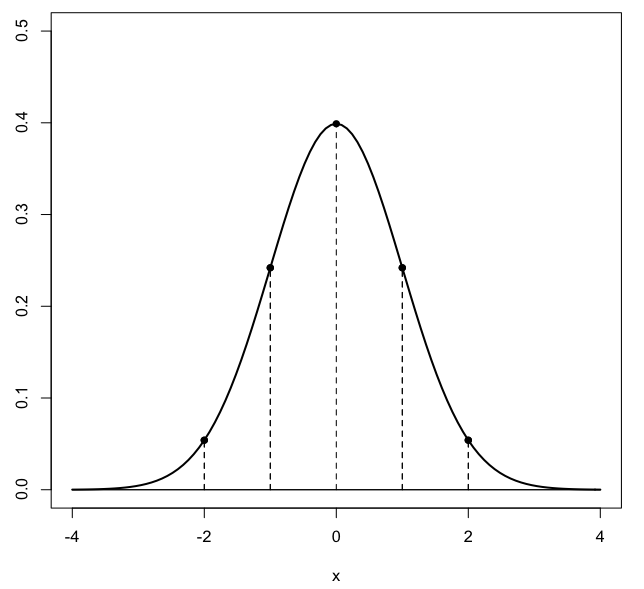
\includegraphics [scale=0.4] {gauss3.png} \end{center}
\begin{document}
\maketitle
\Large
The function
\[ f(x,y) = \frac{x^2}{x^2 + y^2} \]
has some problems:  first, it is not defined at the origin $(0,0)$ but also, as we approach the origin along the $x$-axis and the $y$-axis we get different limiting values, namely
\[ f(x,0) = \frac{x^2}{x^2} = 1 \]
\[ f(0,y) = \frac{0}{y^2} = 0 \]

Rewriting it in polar coordinates ($x = r \cos \theta, r^2 = x^2 + y^2$):
\[ f(r,\theta) = \frac{r^2 \cos^2 \theta}{r^2} = \cos^2 \theta \]

Shankar says:  the function $f$ is generally a function of \emph{two} complex variables, $z$ and its complex conjugate:
\[ z = x + iy \]
\[ z* = x - iy \]
which can be written in terms of $x$ and $y$ as
\[ x = \frac{z + z*}{2} \]
\[ y = \frac{z - z*}{2i} \]
Generally, the value of $f$ depends on both $z$ and $z*$, but we will be very interested in functions which depend only on $z$ and not $z*$.  The reason for this is that only such functions have the property that the derivative at a point does not depend on the direction from which we approach that point.

Consider the function:
\[ f(x,y) = x^2 - y^2 \]
\[ = \frac{(z+z*)^2}{4} + \frac{(z-z*)^2}{4} \]
\[ = \frac{1}{4} \ [ \ z^2 + 2zz* + z*^2 + z^2 - 2zz* + z*^2 \ ] \]
\[ = \frac{z^2 + z*^2}{2} \]
This function is not a function only of $z$ but of both $z$ and $z*$.

We say that $f$ is an \emph{analytic} function of $z$ if it does not depend on $z*$.  Shankar says this means that "$x$ and $y$ enter $f$ \emph{only} in the combination $x + iy$".

The famous Cauchy-Riemann Equations (CRE) are true for $f \iff f$ is an analytic function of $z$.  

For:
\[ f(x,y) = u(x,y) + iv(x,y) \]
The CRE conditions are:
\[ u_x = v_y \]
\[ u_y = -v_x \]

Consider:
\[ f(x,y) = x^2 - y^2 + i2xy \]
CRE requires
\[ u_x = 2x \stackrel{?}{=}  v_y = 2x \]
\[ v_x = 2y \stackrel{?}{=} - u_y = 2y \]
The function is analytic.  As Shankar says, this is expected because:
\[ x^2 - y^2 + 2ixy = (x + iy)(x + iy) = z^2 \]

Consider:
\[ f(x,y) = \cos y - i \sin y \]
CRE requires:
\[ u_x = 0 \stackrel{?}{=} v_y = - \cos y \]
\[ v_x = 0 \stackrel{?}{=}  -u_y = - \sin y \]
This is "impossible" since there is no $y$ that satisfies both of the conditions.  And it's not surprising since
\[ y = \frac{z - z*}{2i} \]

Consider:
\[ f(x,y) = x^2 + y^2 \]
CRE requires:
\[ u_x = 2x \stackrel{?}{=}  v_y = 2y \]
\[ u_y = 0 \stackrel{?}{=}  -v_x \]
CRE are only satisfied if $x=y$.  Also not surprising since
\[ x^2 + y^2 = zz* \]

Consider:
\[ f(x,y) = x^2 - y^2 \]
CRE requires:
\[ u_x = 2x \stackrel{?}{=} v_y = -2y \]
which is true if $x = y$.
\[ u_y = 0 \stackrel{?}{=} -v_x = 0 \]
But "no importance is given to functions which obey the CRE only at isolated points or on lines."

Consider:
\[ f(x,y) = e^x \cos y + i e^x \sin y \]
CRE requires:
\[ u_x = e^x \cos y \stackrel{?}{=} v_y = e^x \cos y \]
\[ u_y = -e^x \sin y \stackrel{?}{=} -v_x = - \sin y e^x \]
Both are true, so this one does satisfy CRE.

Shankar doesn't mention it here but the last function is special, it is $f(z) = e^z$:
\[ e^x \cos y + i e^x \sin y \]
\[ = e^x (\cos y + i \sin y) \]
\[ = e^x e^{iy} \]
\[ = e^{x + iy} \]
\[ = e^z \]
and we did this one in the previous section.

For functions of interest, it may often be true that CRE fails at particular points called \emph{singularities}.

Consider:
\[ f(x,y) = \frac{1}{z} = \frac{z*}{zz*} = \frac{x-iy}{x^2 + y^2} \]
We need:
\[ u_x = \frac{d}{dx} \ \frac{x}{x^2 + y^2} = \frac{x^2 + y^2 - 2x^2}{(x^2 + y^2)^2}  = \frac{y^2 - x^2}{(x^2 + y^2)^2} \]
\[ v_y = \frac{d}{dy} \ (-\frac{y}{x^2 + y^2} ) = - \frac{x^2 - y^2}{(x^2 + y^2)^2} = u_x \]
\[ u_y =  0 = v_x \]
But the function blows up at the origin.  This described by saying it has a pole at the origin.
The function
\[ f(z) = \frac{c}{z} \]
where $c$ is a constant, also blows up at the origin.  We say that the \emph{residue} of the pole at the origin is $c$.

\end{document}  